In order to measure the performance of the different systems the \textit{Equal Error Rate} metric
is chosen. As its name suggests, the \textit{EER} prioritizes in an equal manner the
\textit{false acceptance rate} and the \textit{false rejection rate}. This metric was already used
in the previous works of the current line of investigation related to pronunciation assessment
at phone level \cite{detection_phone_level_mispronunciation_learning, main}, so the same approach
was taken in the present work.

The \textit{EER} can be easily explained by using other important concept related to
performance measures of machine learning classifiers: the \textit{Receiving Operating Characteristic} curve.
So in first place a briefly explanation of the \textit{ROC} curve will be given, and after that
the explanation of the \textit{EER} will be expanded a little bit more.

\subsection{Receiving Operating Characteristic}

% The \textit{ROC} curve of a binary classifier is a plot of the \textit{true positive rate}
% or \textit{sensitivity} as function of the \textit{false positive rate} (or 1 -
% \textit{specificity}), when varying a discrimination threshold and gives an idea of
% how well the system can correctly detect positive instances (sensitivity)
% at expenses of raising false alarms.
The \textit{Receiving Operating Characteristic} (ROC) curve of a binary classifier is a plot
that resumes information of how
well a model can correctly detect positive instances at expenses of raising false alarms
after being tested against a data set.

When testing a given classifier on a dataset the results can be resumed in a particular table
known as \textit{confusion matrix}:

\begin{center}
    \begin{tabular}{ | l | l | l | l | }
    \hline
    & \multicolumn{2}{  c | }{\textbf{Actual Class}} & \\ \hline
    \textbf{Predicted Class} & \textit{Actual Positive} & \textit{Actual Negative} & \textit{Total Count} \\ \hline
    \textit{Predicted Positive} & True Positive (TP) & False Positive (FP) & Total Positives (P) \\ \hline
    \textit{Predicted Negative} & False Negative (FN) & True Negative (TN) & Total Negatives (N) \\ \hline
    \end{tabular}
\end{center}

\textit{True Positive Rate} is calculated as the number of instances predicted
as \textit{positive} which
actually are \textit{positive} over the total number of \textit{positives} while
\textit{False Positive Rate} is calculated as the number of instances predicted as
\textit{positive} which actually are negative:

\begin{multicols}{2}
  \noindent
  \begin{equation}
    \label{eq:tpr}
    TPR = \frac{TP}{P}
  \end{equation}
  \begin{equation}
    \label{eq:fpr}
    FPR = \frac{FP}{N}
  \end{equation}
\end{multicols}

In a \textit{ROC} curve the \textit{TPR} is plotted in function of the \textit{FPR} for
different cut-off points. Each point of the curve represents a {\textit{FPR},\textit{FPR}}
pair corresponding to a particular decision threshold. A test with perfect discrimination
(no overlap between the positives and negatives distributions) would have a \textit{ROC}
curve that passes through the top left corner. So the closer the \textit{ROC} curve is to
the upper left corner, the higher the overall accuracy of the test.

\begin{figure}[H]
  \centering
  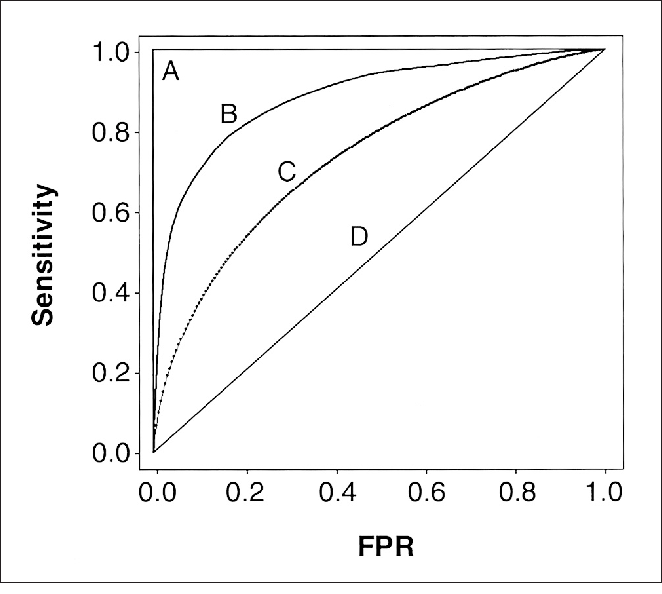
\includegraphics[width=0.5\textwidth]{files/figures/method/roc-curve}
  \caption{ROC curve example. The closer the curve to the upper left corner, the higher the
  accuracy of the system}
  \label{fig:rocCurve}
\end{figure}

\subsection{Equal Error Rate}

\textit{TPR} (Eq. \ref{eq:tpr}) is also called \textit{sensitivity} in the sense that measures
the capacity of the system of detecting positive instances and classifying them
correctly as positives.
At the same time, \textit{specificity} is a measure of the capacity of the system of
avoid raising false alarms, when classifiyng instances that actually belongs to the
negative class. Or, in other words, the capacity of the system of detecting negative
instances and classifying them correctly as negatives. \textit{FPR} (Eq. \ref{eq:fpr})
is actually the complement of \textit{specificity}:

\begin{equation}
specificity = \frac{TN}{N} = \frac{TN}{TN+FP} = 1 - \frac{FP}{TN+FP} = 1 - FPR
\end{equation}

\textit{Equal Error Rate} (EER) is the value on which \textit{sensitivity} is equal to
\textit{specificity}. At this point the system classifies correctly positive instances
as well as it classifies negative instances, thus prioritizing both classes in the same
way. It can be calculated easily as the point of intersection between the \textit{ROC}
curve and the \textit{specificity} curve: $1-FPR$

\begin{figure}[H]
  \centering
  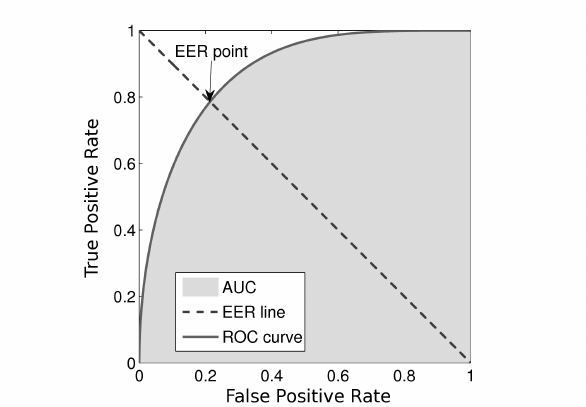
\includegraphics[width=0.5\textwidth]{files/figures/method/eer}
  \caption{EER is equal to the value of the intersection between the ROC curve and
  the Sensitivty curve as function of \textit{FPR}}
  \label{fig:eer}
\end{figure}

\textit{EER} is a proper performance measure for the task of pronunciation assessment
at phone level because both correctly pronounced and mispronounced
classes are equally important. In other tasks, such as \textit{Bank Fraud} or
\textit{Spam Detection}, it may be essential to strictly prioritize one class over the
other. In the current task however it is reasonable to assign the same priority
to both \textit{sensitivity} and \textit{specificity}.
Anyway, it is worth mentioning that during language learning a student may get
discouraged if she pronounces an utterance correctly and the system classifies it as
an error. A threshold can be chosen in order to ensure that whenever the system
classifies an instance as incorrect it has an acceptable level of confidence.

